\subsection{SCENARIO}
\begin{figure}
\begin{center}
  \begin{tabular}{@{\hspace{0.1cm}}c}
		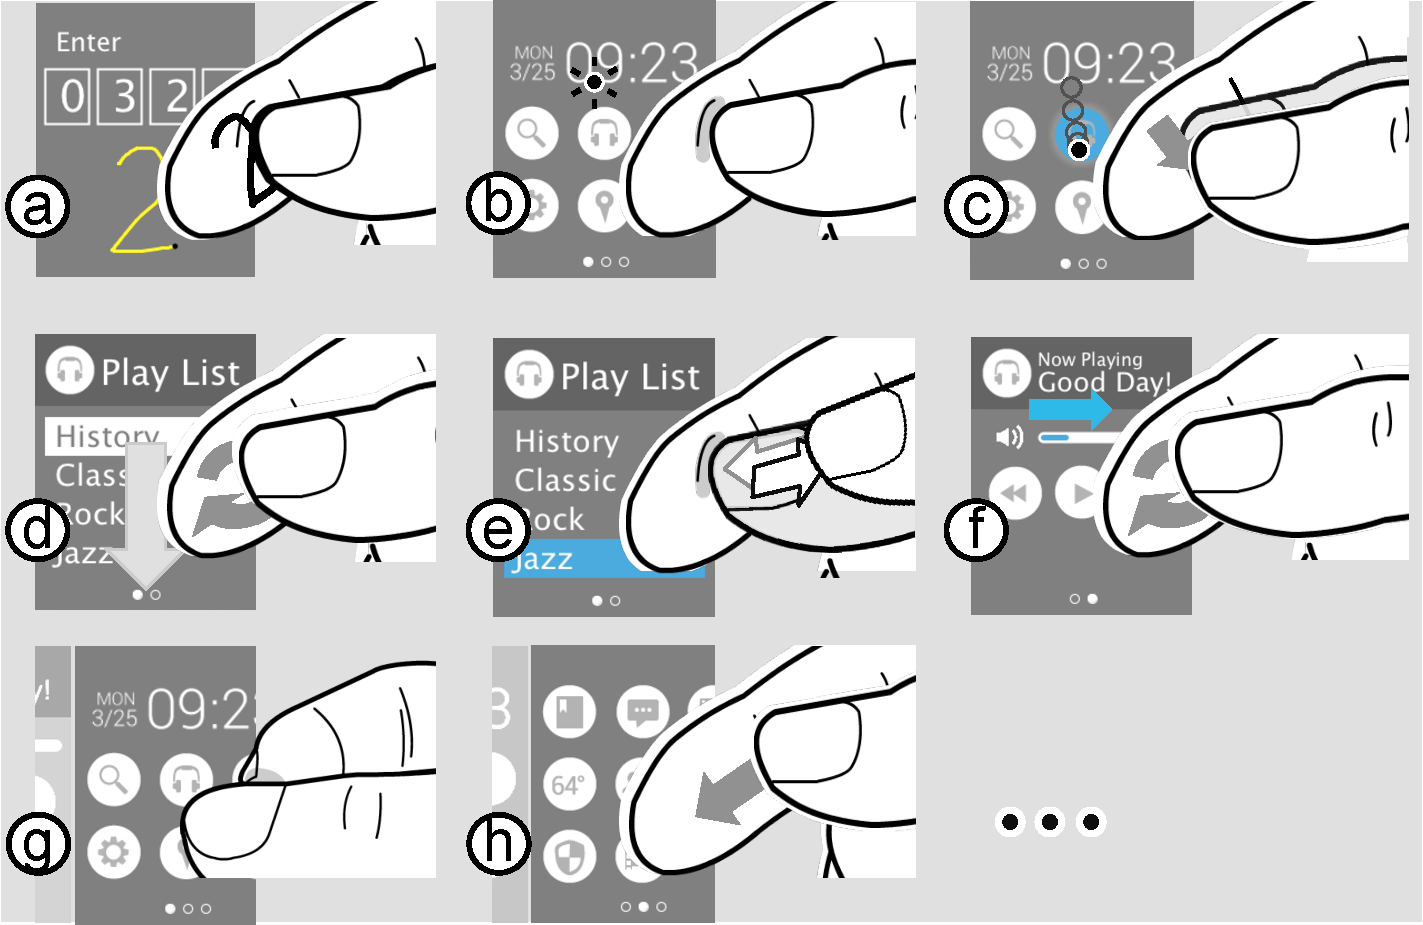
\includegraphics[width=1\linewidth]{walkthrough4}\\
   \end{tabular}
\caption{The walkthrough illustrates the use of FingerPad for glass displays. The graphics on the left-hand side of the subfigures are GUIs presented in the glass display view. The graphics on the right-hand side of the subfigures are the suggested gestures that can be enabled through our technique. }
\label{fig:walkthrough}
\end{center}
\end{figure}

Figure \ref{fig:walkthrough} illustrates a scenario of FingerPad for private visual outputs, such as the glass-mounted displays.
On the train on his way to work, Robin puts on the glass display. 
On the screen, the glass asks Robin the password for authentication. Instead of using voice input, he chooses to use the FingerPad input for privacy concern. 
(a) He writes four numbers, one by one, on his index fingertip, to unlock the glass application. 
(b) Robin long presses on the index fingertip to enter the cursor mode, (c) moves the cursor over the music app, and takes off the thumb for selection.
(d) In the music list, he circles on the fingertip to move to jazz category, and (e) clicks to enter the player page. (f) He circles again to tune up the volume. (g) To jump to home screen, he taps on the tip of the index finger. Now, he swipes the thumb leftward, moving to next app pages and plans to check the schedule of the day.

%(a) The user wrote password words on the fingertip to unlock the glass display, (b) long pressed to enter the cursor mode, (c) moved over music app, and taken-off for selection. (d) Circling on the fingertip, the user pulled down the list until Jazz, (e) single clicked to enter the player page. (f) After playing the music, he tuned up the volume by circling. (g) Tapping on the very end of the fingertip bring the display to home screen. (h) He slid leftward to second page, and started to check schedules of the day.